% Provenance (never printed): cycle 3 / 6e "La planete Terre" (water in the
% ground, groundwater, springs and wells; resource); see
% sources/book1/PROVENANCE.md. Book 1, grade 6, chapter 5.
% Vocabulary guard: "sediment" not before g7.4; the water cycle is recalled
% from the physics book (prose only).
\chapter{Water onder de grond}\label{ch:g6:water-underground}

Op een hete zomerdag zijn de akkers droog en staan de beken laag. Toch
blijft er aan de voet van een \omterm{def:g1:landscapes-around-us:landform}{heuvel} water uit de grond opwellen, koud en
helder, zoals de hele winter, en het vult een vijver. Het heeft al weken
niet geregend. Waar komt dit water vandaan, en hoe komt het uit het
\omterm{def:g3:stones-pebbles-sand:rock}{gesteente}?

\begin{omfigure}
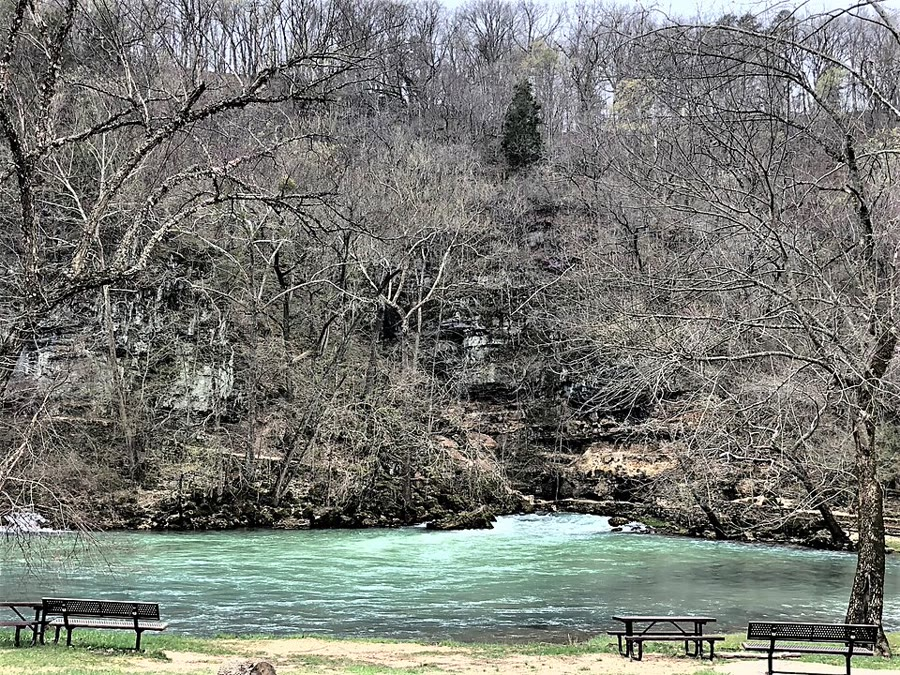
\includegraphics[width=0.72\linewidth]{images/book1/g6-big-spring.jpg}

{\small Een \omterm{def:g6:water-underground:spring}{bron} welt op aan de voet van een rotswand en vult een vijver:
Big Spring, Missouri (Verenigde Staten). (Foto: Johnston9494, CC BY-SA 4.0,
via Wikimedia Commons.)}
% ledger: commons:big-spring
\end{omfigure}

\begin{recall}
Bijna al het water op Aarde is \omterm{def:g2:water-on-earth:salt-fresh}{zout water}; \omterm{def:g2:water-on-earth:salt-fresh}{zoet water} is een klein deel,
dat vooral als ijs en onder de grond is opgeslagen
(\cref{ch:g2:water-on-earth}). \omterm{def:g3:stones-pebbles-sand:rock}{Gesteenten} zoals zandsteen en kalksteen
bestaan uit korrels of schelpen die aan elkaar vastzitten, terwijl klei en
schalie uit heel fijne deeltjes bestaan (\cref{ch:g6:rocks-and-minerals}).
In het natuurkundeboek heb je het water gevolgd in de waterkringloop: het
verdampt uit de \omterm{def:g2:water-on-earth:ocean}{zeeën}, condenseert tot \omterm{def:g4:clouds-rain-snow:cloud}{wolken} en valt terug als \omterm{def:g4:clouds-rain-snow:precipitation}{regen} of
\omterm{def:g4:clouds-rain-snow:precipitation}{sneeuw}.
\end{recall}

\section{Regen zakt in de grond}

Als er \omterm{def:g4:clouds-rain-snow:precipitation}{regen} op het land valt, kan het water drie wegen nemen. Een deel
verdampt weer in de lucht. Een deel stroomt over het oppervlak, de
hellingen af, naar beken en \omterm{def:g1:landscapes-around-us:water}{rivieren}: dat is \emph{afstroming}. De rest
zakt in de grond.

\begin{definition}[Infiltratie]\label{def:g6:water-underground:infiltration}
\emph{Infiltratie}\index{infiltratie} is het wegzakken van regenwater, of
gesmolten \omterm{def:g4:clouds-rain-snow:precipitation}{sneeuw}, in de grond, door de bodem heen en omlaag in het
\omterm{def:g3:stones-pebbles-sand:rock}{gesteente}.
\end{definition}

Hoeveel water er in de grond zakt, hangt af van de grond. Op een steile
helling, op kale of harde grond, op een weg of een parkeerplaats, of als de
bodem al doorweekt is, stroomt het meeste water weg. Op een flauwe helling,
onder gras en bomen, op zandgrond, heeft meer water de tijd om in de grond
te zakken.

\begin{omfigure}
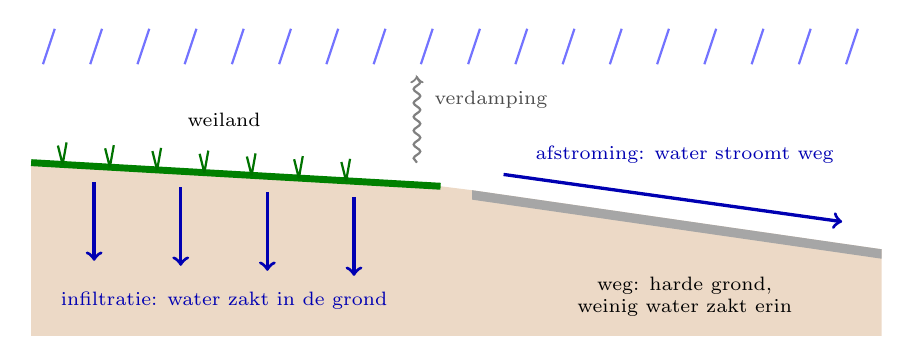
\begin{tikzpicture}[x=1cm, y=1cm]
  % rain
  \foreach \x in {0.3,0.9,...,10.5} \draw[blue!55, thick] (\x,3.9) -- (\x-0.15,3.45);
  % ground: field on the left (gentle), road and town on the right
  \fill[brown!30] (0,0) -- (0,2.2) -- (5.2,1.9) -- (5.6,1.85) -- (10.8,1.1) -- (10.8,0) -- cycle;
  \draw[green!50!black, line width=2.5pt] (0,2.2) -- (5.2,1.9);
  \fill[gray!70] (5.6,1.85) -- (10.8,1.1) -- (10.8,0.98) -- (5.6,1.73) -- cycle;
  \foreach \x in {0.4,1.0,...,4.6} \draw[green!45!black, thick] (\x,{2.2-0.058*\x}) -- ++(0.05,0.28) (\x,{2.2-0.058*\x}) -- ++(-0.06,0.24);
  % infiltration arrows in the field
  \foreach \x in {0.8,1.9,3.0,4.1} \draw[->, blue!70!black, very thick] (\x,{2.0-0.058*\x}) -- ++(0,-1.0);
  \node[font=\scriptsize, blue!70!black, align=center, fill=brown!30] at (2.45,0.45) {infiltratie: water zakt in de grond};
  % run-off on the road
  \draw[->, blue!70!black, very thick] (6.0,2.05) -- (10.3,1.45);
  \node[font=\scriptsize, blue!70!black, align=center] at (8.3,2.3) {afstroming: water stroomt weg};
  \node[font=\scriptsize, align=center] at (8.3,0.5) {weg: harde grond,\\ weinig water zakt erin};
  \node[font=\scriptsize] at (2.45,2.75) {weiland};
  % evaporation
  \draw[->, gray, thick, decorate, decoration={snake, amplitude=1.2pt, segment length=5pt}] (4.9,2.2) -- (4.9,3.3);
  \node[font=\scriptsize, gray!60!black, anchor=west] at (5.0,3.0) {verdamping};
\end{tikzpicture}

{\small De drie wegen van regenwater. In het weiland zakt veel ervan in de
grond; op de weg stroomt het meeste weg.}
\end{omfigure}

\section{Poreuze en doorlatende gesteenten}

Bekijk een handvol droog \omterm{def:g3:stones-pebbles-sand:sand}{zand} door een loep: tussen de korrels zitten
piepkleine lege ruimtes. Giet er water op en het water vult die ruimtes.
Veel \omterm{def:g3:stones-pebbles-sand:rock}{gesteenten} zijn zo: ze zitten vol kleine gaatjes tussen hun korrels,
of vol dunne scheurtjes.

\begin{definition}[Porositeit]\label{def:g6:water-underground:porosity}
De \emph{poriën}\index{porie} van een \omterm{def:g3:stones-pebbles-sand:rock}{gesteente} zijn de lege ruimtes
tussen de korrels en in de scheurtjes. Een \omterm{def:g3:stones-pebbles-sand:rock}{gesteente} met poriën is
\emph{poreus}\index{poreus}. De \emph{porositeit}\index{porositeit} is het
deel van het volume dat uit poriën bestaat, geschreven als percentage.
\end{definition}

\begin{definition}[Doorlatendheid]\label{def:g6:water-underground:permeability}
Een \omterm{def:g3:stones-pebbles-sand:rock}{gesteente} is \emph{doorlatend}\index{doorlatend} als water erdoorheen
kan stromen, omdat de \omterm{def:g6:water-underground:porosity}{poriën} groot genoeg zijn en met elkaar in verbinding
staan. Het is \emph{ondoorlatend}\index{ondoorlatend} als er geen water
doorheen kan stromen. De \emph{doorlatendheid}\index{doorlatendheid} is hoe
makkelijk water door een \omterm{def:g3:stones-pebbles-sand:rock}{gesteente} stroomt.
\end{definition}

De twee begrippen zijn niet hetzelfde. Klei is heel \omterm{def:g6:water-underground:porosity}{poreus}: de helft van
het volume bestaat uit \omterm{def:g6:water-underground:porosity}{poriën}. Maar die \omterm{def:g6:water-underground:porosity}{poriën} zijn zo piepklein dat het
water erin vast blijft zitten: klei is \emph{\omterm{def:g6:water-underground:permeability}{ondoorlatend}}. \omterm{def:g3:stones-pebbles-sand:sand}{Zand} heeft
minder \omterm{def:g6:water-underground:porosity}{poriën} dan klei, maar ze zijn wijd en staan met elkaar in
verbinding: \omterm{def:g3:stones-pebbles-sand:sand}{zand} is \emph{\omterm{def:g6:water-underground:permeability}{doorlatend}}. Graniet zonder scheuren heeft bijna
helemaal geen \omterm{def:g6:water-underground:porosity}{poriën}.
% ledger: heath:porosity

\begin{omfigure}
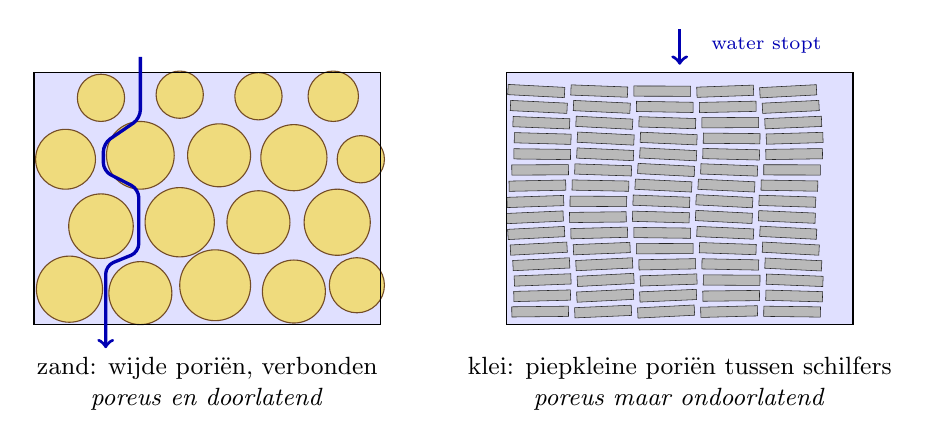
\begin{tikzpicture}
  % sand
  \begin{scope}
    \fill[blue!12] (0,0) rectangle (4.4,3.2);
    \foreach \x/\y/\r in {0.45/0.45/0.42, 1.35/0.4/0.4, 2.3/0.5/0.45, 3.3/0.42/0.4, 4.1/0.5/0.35,
                         0.85/1.25/0.41, 1.85/1.3/0.44, 2.85/1.3/0.4, 3.85/1.3/0.42,
                         0.4/2.1/0.38, 1.35/2.15/0.43, 2.35/2.15/0.4, 3.3/2.12/0.42, 4.15/2.1/0.3,
                         0.85/2.88/0.3, 1.85/2.92/0.3, 2.85/2.9/0.3, 3.8/2.9/0.32}
      \fill[yellow!55!brown!60, draw=brown!60!black] (\x,\y) circle (\r);
    \draw (0,0) rectangle (4.4,3.2);
    \draw[->, blue!70!black, very thick, rounded corners=3pt] (1.35,3.4) -- (1.35,2.62) -- (0.88,2.3) -- (0.88,1.95) -- (1.33,1.72) -- (1.33,0.92) -- (0.91,0.75) -- (0.91,-0.3);
    \node[font=\small, align=center] at (2.2,-0.75) {zand: wijde poriën, verbonden\\ \emph{poreus en doorlatend}};
  \end{scope}
  % clay
  \begin{scope}[xshift=6.0cm]
    \fill[blue!12] (0,0) rectangle (4.4,3.2);
    \foreach \y in {0.1,0.3,...,3.0}
      \foreach \x in {0.05,0.85,...,3.7}
        \fill[gray!55, draw=gray!30!black, line width=0.2pt, rotate around={{3*sin(57*\x+91*\y)}:(\x+0.36,\y+0.06)}]
          ({\x+0.05*sin(200*\y)},\y) rectangle ++(0.72,0.13);
    \draw (0,0) rectangle (4.4,3.2);
    \draw[->, blue!70!black, very thick] (2.2,3.75) -- (2.2,3.3);
    \node[font=\scriptsize, blue!70!black] at (3.3,3.55) {water stopt};
    \node[font=\small, align=center] at (2.2,-0.75) {klei: piepkleine poriën tussen schilfers\\ \emph{poreus maar ondoorlatend}};
  \end{scope}
\end{tikzpicture}

{\small De \omterm{def:g6:water-underground:porosity}{poriën} (in blauw) tussen de korrels van een \omterm{def:g3:stones-pebbles-sand:sand}{zand} en tussen de
schilfers van een klei, sterk vergroot. Water vindt een weg door het \omterm{def:g3:stones-pebbles-sand:sand}{zand};
in de klei blijft het vastzitten.}
\end{omfigure}

De tabel geeft de \omterm{def:g6:water-underground:porosity}{porositeit} van een paar materialen, en het deel van het
water dat er vanzelf uit wegloopt als ze vol water zitten. De rest blijft
aan de korrels vastzitten.

\begin{center}\small
\begin{tabular}{|l|c|c|}
\hline
\textbf{materiaal} & \textbf{\omterm{def:g6:water-underground:porosity}{porositeit} (\%)} & \textbf{water dat wegloopt (\%)} \\
\hline
bodem & 55 & 40 \\
klei & 50 & 2 \\
\omterm{def:g3:stones-pebbles-sand:sand}{zand} & 25 & 22 \\
\omterm{def:g3:stones-pebbles-sand:pebble}{grind} & 20 & 19 \\
kalksteen & 20 & 18 \\
zandsteen & 11 & 6 \\
graniet & 0.1 & 0.09 \\
\hline
\end{tabular}
\end{center}
% ledger: heath:porosity

\begin{method}[Hoeveel water houdt een gesteente vast?]\label{met:g6:water-underground:volume}
\begin{enumerate}
  \item Zoek het volume van het \omterm{def:g3:stones-pebbles-sand:rock}{gesteente} (voor een blok: lengte $\times$ breedte
        $\times$ hoogte).
  \item Vermenigvuldig met de \omterm{def:g6:water-underground:porosity}{porositeit} en deel door 100: dat is het
        volume van de \omterm{def:g6:water-underground:porosity}{poriën}, dus het water dat het \omterm{def:g3:stones-pebbles-sand:rock}{gesteente} bevat als het
        vol zit.
  \item Gebruik voor het water dat wegloopt het tweede percentage op
        dezelfde manier. (1~kubieke meter is 1000~liter.)
\end{enumerate}
\end{method}

\begin{example}[Een kubieke meter zand]\label{ex:g6:water-underground:sand}
Een kubieke meter \omterm{def:g3:stones-pebbles-sand:sand}{zand} die vol water zit, bevat $1000 \times 25 \div 100 =
250$~liter water in zijn \omterm{def:g6:water-underground:porosity}{poriën}. Daarvan loopt $1000 \times 22 \div 100 = 220$
liter vanzelf weg; 30~liter blijft aan de korrels vastzitten. Een kubieke
meter klei bevat twee keer zoveel water, 500~liter, maar er loopt maar
20~liter uit weg.
% ledger: heath:porosity
\end{example}

\begin{inthelab}[Zand of klei? (in de klas, met de leraar)]
Twee bloempotten met een gat in de bodem staan boven twee glazen. De ene
is gevuld met droog \omterm{def:g3:stones-pebbles-sand:sand}{zand}, de andere met droge, aangedrukte kleigrond. De
leraar giet tegelijk in elke pot hetzelfde glas water. Door het \omterm{def:g3:stones-pebbles-sand:sand}{zand}
druppelt het water al snel in het glas eronder. Op de klei blijft het
water bovenop staan als een plas en komen er maar een paar druppels door,
langzaam: het \omterm{def:g3:stones-pebbles-sand:sand}{zand} is \omterm{def:g6:water-underground:permeability}{doorlatend}, de klei niet.
\end{inthelab}

\section{Grondwater en de grondwaterspiegel}

Graaf een kuil in het \omterm{def:g3:stones-pebbles-sand:sand}{zand} van een strand, een paar stappen van de \omterm{def:g2:water-on-earth:ocean}{zee}: na
een tijdje verschijnt er water op de bodem van de kuil. Je hebt de plek
bereikt waar alle \omterm{def:g6:water-underground:porosity}{poriën} van het \omterm{def:g3:stones-pebbles-sand:sand}{zand} vol water zitten.
% ledger: wss:aquifer

\begin{definition}[Grondwater]\label{def:g6:water-underground:groundwater}
\emph{Grondwater}\index{grondwater} is het water onder de grond dat de
\omterm{def:g6:water-underground:porosity}{poriën} en scheuren van de bodem en van de \omterm{def:g3:stones-pebbles-sand:rock}{gesteenten} vult.
\end{definition}

\begin{definition}[Grondwaterspiegel]\label{def:g6:water-underground:water-table}
Onder een bepaalde diepte zitten alle \omterm{def:g6:water-underground:porosity}{poriën} van het \omterm{def:g3:stones-pebbles-sand:rock}{gesteente} vol water.
De \emph{grondwaterspiegel}\index{grondwaterspiegel} is de bovenkant van
deze met water gevulde zone. Erboven bevatten de \omterm{def:g6:water-underground:porosity}{poriën} lucht en een
beetje water; eronder zitten ze vol water.
% ledger: wss:aquifer
\end{definition}

De \omterm{def:g6:water-underground:water-table}{grondwaterspiegel} is niet vlak. Hij volgt de vorm van het land, maar
vlakker: hoger onder de \omterm{def:g1:landscapes-around-us:landform}{heuvels}, lager onder de \omterm{def:g1:landscapes-around-us:landform}{dalen}. Hij gaat ook met de
seizoenen op en neer. Na een regenseizoen heeft de \omterm{def:g4:clouds-rain-snow:precipitation}{regen} die in de grond is
gezakt hem omhoog gebracht; na een lang droog seizoen stroomt het water
langzaam weg naar bronnen en \omterm{def:g1:landscapes-around-us:water}{rivieren}, en zakt de \omterm{def:g6:water-underground:water-table}{grondwaterspiegel}.

\omterm{def:g6:water-underground:groundwater}{Grondwater} is een grote voorraad \omterm{def:g2:water-on-earth:salt-fresh}{zoet water}. Van al het zoete water op
Aarde is ongeveer 69~\% ijs en eeuwige \omterm{def:g4:clouds-rain-snow:precipitation}{sneeuw}, en ongeveer 30~\% \omterm{def:g6:water-underground:groundwater}{grondwater};
het zoete water van alle \omterm{def:g1:landscapes-around-us:water}{meren} samen is maar ongeveer een kwart procent.
Er is meer dan honderd keer zoveel \omterm{def:g6:water-underground:groundwater}{grondwater} als \omterm{def:g2:water-on-earth:salt-fresh}{zoet water} in de \omterm{def:g1:landscapes-around-us:water}{meren}.
% ledger: wss:fresh-shares

\begin{omfigure}
\begin{tikzpicture}
  \begin{axis}[xbar, width=0.8\linewidth, height=3.9cm, bar width=8pt,
      xmin=0, xmax=85, ymin=-0.6, ymax=4.6, y dir=reverse,
      ytick={0,...,4}, yticklabels={{ijs en eeuwige sneeuw},{grondwater},{bodemijs en permafrost},{meren},{al het andere}},
      xlabel={procent van al het zoete water op Aarde},
      axis x line=bottom, axis y line=left, axis line style={-},
      tick label style={font=\scriptsize}, label style={font=\small},
      nodes near coords, nodes near coords style={font=\scriptsize, anchor=west},
      point meta=explicit symbolic, enlarge y limits=false, clip=false]
    \addplot[fill=blue!35, draw=blue!60!black] table[x=pct, y=idx, meta=pct] {figdata/out/grade-6-water_table-fresh.dat};
  \end{axis}
\end{tikzpicture}

{\small Waar het zoete water van de Aarde zit. De staven voor de \omterm{def:g1:landscapes-around-us:water}{meren} en
voor al het andere (\omterm{def:g1:landscapes-around-us:water}{rivieren}, de lucht, de bodem, moerassen, levende
wezens) zijn te kort om te zien.}
% ledger: wss:fresh-shares (figdata/grade-6/water_table.py, part fresh)
\end{omfigure}

\section{Bronnen en putten}

\begin{definition}[Bron en put]\label{def:g6:water-underground:spring}
Een \emph{bron}\index{bron (van grondwater)} is een plek waar \omterm{def:g6:water-underground:groundwater}{grondwater}
vanzelf uit de grond komt, waar de \omterm{def:g6:water-underground:water-table}{grondwaterspiegel} het oppervlak raakt.
Een \emph{put}\index{put} is een gat dat tot onder de \omterm{def:g6:water-underground:water-table}{grondwaterspiegel} is
gegraven of geboord, zodat \omterm{def:g6:water-underground:groundwater}{grondwater} de bodem ervan vult en eruit kan
worden opgehaald.
\end{definition}

De doorsnede hieronder loopt door een \omterm{def:g1:landscapes-around-us:landform}{dal} van de Varden Hills, het gebied
van onze oefeningen. De \omterm{def:g1:landscapes-around-us:landform}{heuvels} bestaan uit krijt, een witte, zachte,
poreuze en doorlatende kalksteen. Onder het krijt ligt een laag schalie,
die \omterm{def:g6:water-underground:permeability}{ondoorlatend} is. De \omterm{def:g4:clouds-rain-snow:precipitation}{regen} zakt in het krijt, vult de \omterm{def:g6:water-underground:porosity}{poriën} en stopt
op de schalie.

\begin{omfigure}
\begin{tikzpicture}
\begin{axis}[omsection, width=0.95\linewidth, height=7.2cm,
    xmin=0, xmax=2.8, ymin=0, ymax=560,
    xlabel={afstand vanaf het zuideinde van de doorsnede (km)},
    ylabel={hoogte boven zeeniveau (m)},
    tick label style={font=\scriptsize}, label style={font=\small},
    clip mode=individual]
  \addplot[om lith={icsJurassic!40}{om limestone}, draw=black, line width=0.3pt, even odd rule] table {figdata/out/grade-6-water_table-unit-limestone.dat};
  \addplot[om lith={icsJurassic!15}{om shale}, draw=black, line width=0.3pt, even odd rule] table {figdata/out/grade-6-water_table-unit-shale.dat};
  \addplot[om lith={icsCretaceous!35}{om limestone}, draw=black, line width=0.3pt, even odd rule] table {figdata/out/grade-6-water_table-unit-chalk.dat};
  \addplot[lith alluvium, draw=black, line width=0.3pt, even odd rule] table {figdata/out/grade-6-water_table-unit-alluvium.dat};
  \addplot[black, thick] table {figdata/out/grade-6-water_table-ground.dat};
  \addplot[blue!75!black, very thick] table {figdata/out/grade-6-water_table-wet.dat};
  \addplot[blue!75!black, very thick, dashed] table {figdata/out/grade-6-water_table-dry.dat};
  % wells
  \addplot[fill=white, draw=black, line width=0.4pt] table {figdata/out/grade-6-water_table-well-rects.dat};
  \addplot[only marks, mark=none, point meta=explicit symbolic, nodes near coords,
    nodes near coords style={font=\scriptsize\bfseries, anchor=south east, fill=white, fill opacity=0.8, text opacity=1, inner sep=1pt}]
    table[x=s_km, y=z_m, meta=label, row sep=\\] {s_km z_m label\\ 1.45 401.3 put~A\\ 1.7 470.3 put~B\\ };
  % river and spring
  \addplot[only marks, mark=*, mark size=2.2pt, blue!75!black] table[x=s_km, y=z_m] {figdata/out/grade-6-water_table-points.dat};
  \node[font=\scriptsize, blue!70!black, anchor=south east] at (axis cs:0.215,140) {rivier};
  \node[font=\scriptsize, blue!70!black, anchor=east] at (axis cs:0.83,218) {bron};
  \node[font=\scriptsize] at (axis cs:2.2,470) {krijt (doorlatend)};
  \node[font=\scriptsize, fill=white, fill opacity=0.8, text opacity=1] at (axis cs:2.2,95) {schalie (ondoorlatend)};
  \node[font=\scriptsize, fill=white, fill opacity=0.8, text opacity=1] at (axis cs:0.95,25) {kalksteen};
  \node[font=\scriptsize, blue!70!black, fill=white, fill opacity=0.8, text opacity=1, align=center] at (axis cs:2.15,250) {grondwaterspiegel:\\ na het regenseizoen (doorgetrokken)\\ na het droge seizoen (gestippeld)};
\end{axis}
\end{tikzpicture}

{\small Een noord--zuiddoorsnede door de Varden Hills, van de \omterm{def:g1:landscapes-around-us:water}{rivier} de
noordelijke helling op (hoogten ongeveer 2~keer overdreven). Het water in
het krijt stopt op de schalie en komt naar buiten als \omterm{def:g6:water-underground:spring}{bron} waar de
onderkant van het krijt de helling raakt. \omterm{def:g6:water-underground:spring}{Put}~A bereikt altijd het water;
\omterm{def:g6:water-underground:spring}{put}~B bereikt het alleen na het regenseizoen.}
% (figdata/grade-6/water_table.py; region model figdata/shared/region.py)
\end{omfigure}

De \omterm{def:g6:water-underground:spring}{bron} stroomt waar de onderkant van het krijt de helling raakt: het
water kan niet omlaag door de schalie, dus stroomt het over de bovenkant
van de schalie en komt het op de helling naar buiten. Zolang er water in
het krijt boven de schalie zit, blijft de \omterm{def:g6:water-underground:spring}{bron} stromen, zelfs in een droge
zomer: dat is het antwoord op de vraag aan het begin van het hoofdstuk.

Kijk naar de twee putten. \omterm{def:g6:water-underground:spring}{Put}~A is 100~m diep; de bodem ligt in elk
seizoen onder de \omterm{def:g6:water-underground:water-table}{grondwaterspiegel}, dus geeft hij altijd water. \omterm{def:g6:water-underground:spring}{Put}~B is
nog dieper, 105~m, maar hij is hoger op de \omterm{def:g1:landscapes-around-us:landform}{heuvel} gegraven: de bodem ligt
na het regenseizoen onder de \omterm{def:g6:water-underground:water-table}{grondwaterspiegel} en na het droge seizoen
erboven. In de zomer staat \omterm{def:g6:water-underground:spring}{put}~B droog. Wat telt, is niet hoe diep een \omterm{def:g6:water-underground:spring}{put}
is, maar hoe ver de bodem onder de laagste \omterm{def:g6:water-underground:water-table}{grondwaterspiegel} komt.
% (figdata/grade-6/water_table.py, part wells)

\begin{omfigure}
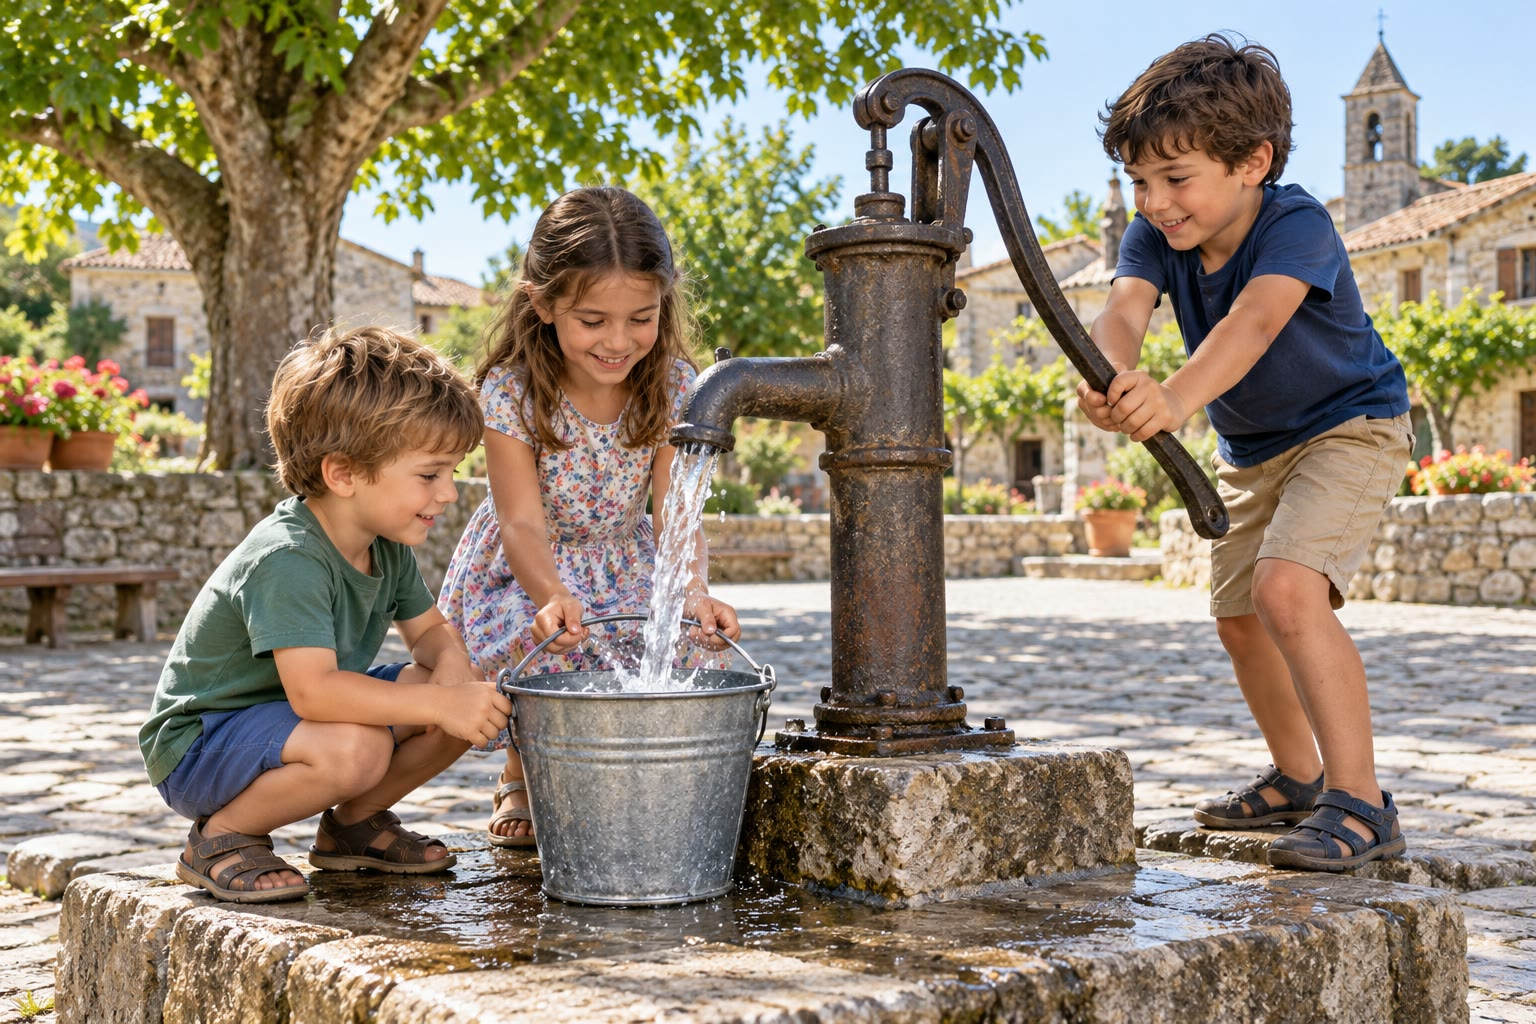
\includegraphics[width=0.6\linewidth]{images/book1/ai/g6-hand-pump.jpg}

{\small Kinderen vullen een emmer bij de handpomp van een dorpsput.
(AI-illustratie.)}
\end{omfigure}

\begin{remark}[Een put kan droog komen te staan]\label{rem:g6:water-underground:pumping}
Water uit een \omterm{def:g6:water-underground:spring}{put} pompen verlaagt de \omterm{def:g6:water-underground:water-table}{grondwaterspiegel} eromheen. Als er
sneller water wordt opgepompt dan de \omterm{def:g4:clouds-rain-snow:precipitation}{regen} het \omterm{def:g3:stones-pebbles-sand:rock}{gesteente} bijvult, zakt de
\omterm{def:g6:water-underground:water-table}{grondwaterspiegel} steeds verder: de \omterm{def:g6:water-underground:spring}{put} geeft steeds minder water en kan
droog komen te staan. Twee buren die uit hetzelfde \omterm{def:g3:stones-pebbles-sand:rock}{gesteente} pompen, delen
hetzelfde water: de ene pomp kan de \omterm{def:g6:water-underground:spring}{put} van de ander droog laten vallen.
% ledger: wss:aquifer
\end{remark}

\section{Watervoerende lagen}

\begin{definition}[Watervoerende laag]\label{def:g6:water-underground:aquifer}
Een \emph{watervoerende laag}\index{watervoerende laag} (of aquifer) is
een laag \omterm{def:g6:water-underground:porosity}{poreus} en \omterm{def:g6:water-underground:permeability}{doorlatend} \omterm{def:g3:stones-pebbles-sand:rock}{gesteente}, vol \omterm{def:g6:water-underground:groundwater}{grondwater}, die dit water
naar bronnen en putten laat stromen. De \omterm{def:g4:clouds-rain-snow:precipitation}{regen} die in de grond zakt, vult
haar weer aan.
% ledger: wss:aquifer
\end{definition}

Het krijt van de Varden Hills is een \omterm{def:g6:water-underground:aquifer}{watervoerende laag}: het is \omterm{def:g6:water-underground:porosity}{poreus}, het
is \omterm{def:g6:water-underground:permeability}{doorlatend}, en de boerderijen op de \omterm{def:g1:landscapes-around-us:landform}{heuvels} halen er hun water uit. De
schalie eronder is geen \omterm{def:g6:water-underground:aquifer}{watervoerende laag}: water kan er niet doorheen
stromen. Nog dieper, onder de schalie, liggen een kalksteen en een
zandsteen, die ook water kunnen bevatten; om dat te bereiken, moet een \omterm{def:g6:water-underground:spring}{put}
dwars door de schalie worden geboord.

\omterm{def:g6:water-underground:groundwater}{Grondwater} hoort bij de waterkringloop. \omterm{def:g4:clouds-rain-snow:precipitation}{Regen} zakt in een \omterm{def:g6:water-underground:aquifer}{watervoerende
laag}; het \omterm{def:g6:water-underground:groundwater}{grondwater} stroomt langzaam door de \omterm{def:g6:water-underground:porosity}{poriën}; het komt naar buiten bij bronnen en in \omterm{def:g1:landscapes-around-us:water}{rivieren}, die het naar de \omterm{def:g2:water-on-earth:ocean}{zee} voeren; daar
verdampt het, en het valt weer als \omterm{def:g4:clouds-rain-snow:precipitation}{regen}. Water uit een \omterm{def:g6:water-underground:aquifer}{watervoerende laag}
halen is als water uit een tank halen die de \omterm{def:g4:clouds-rain-snow:precipitation}{regen} langzaam vult: het
houdt alleen stand als we er niet meer uit halen dan de \omterm{def:g4:clouds-rain-snow:precipitation}{regen} terugbrengt.

\section{Grondwater schoon houden}

Water dat in de grond zakt, wordt onderweg gefilterd: bladeren,
bodemdeeltjes en kleine beestjes worden door de bodem en het \omterm{def:g3:stones-pebbles-sand:rock}{gesteente}
tegengehouden. Daarom ziet water uit een \omterm{def:g6:water-underground:spring}{bron} of een \omterm{def:g6:water-underground:spring}{put} er meestal
kristalhelder uit. Maar stoffen die \emph{opgelost} zijn in het water,
worden niet tegengehouden: ze reizen met het water mee omlaag naar de
\omterm{def:g6:water-underground:water-table}{grondwaterspiegel}.
% ledger: wss:gw-quality

\omterm{def:g6:water-underground:groundwater}{Grondwater} kan bedorven worden door wat mensen op de grond doen: kunstmest
en bestrijdingsmiddelen op akkers en in tuinen, strooizout op gladde
wegen, brandstof die uit een tank lekt, afval dat in de open lucht wordt
gestort, het overlopen van slecht onderhouden beerputten van huizen. Als
die stoffen eenmaal in een \omterm{def:g6:water-underground:aquifer}{watervoerende laag} zijn opgelost, zijn ze
moeilijk te verwijderen, en is het water misschien niet meer veilig om
zonder behandeling te drinken. Daarom moet het water van een \omterm{def:g6:water-underground:spring}{put} worden getest voordat je het drinkt, en kun je kunstmest, brandstof en afval het best ver van putten en bronnen houden.
% ledger: wss:gw-quality

Opgeloste stoffen reizen met het \omterm{def:g6:water-underground:groundwater}{grondwater} mee. Onder de
\omterm{def:g6:water-underground:water-table}{grondwaterspiegel} kruipt het water langzaam bergafwaarts: van waar de
\omterm{def:g6:water-underground:water-table}{grondwaterspiegel} hoog is, onder de \omterm{def:g1:landscapes-around-us:landform}{heuvels}, naar waar hij laag is, bij de
bronnen en de \omterm{def:g1:landscapes-around-us:water}{rivieren}. Iets wat wordt gemorst en in de grond zakt, blijft
dus niet liggen waar het viel. Het zakt naar de \omterm{def:g6:water-underground:water-table}{grondwaterspiegel} en drijft
dan met het \omterm{def:g6:water-underground:groundwater}{grondwater} bergafwaarts mee, naar wat er lager op de helling
ligt.
% ledger: wss:gw-quality, wss:aquifer

\begin{omfigure}
\begin{tikzpicture}[x=1cm, y=1.15cm, font=\scriptsize]
  % ground (the chalk) and the water-filled zone under the water table
  \fill[black!6] (0,0) -- (0,4.090) -- plot[smooth] coordinates {(0.00,4.090) (1.00,4.013) (2.00,3.887) (3.00,3.692) (4.00,3.407) (5.00,3.033) (6.00,2.600) (7.00,2.167) (8.00,1.793) (9.00,1.508) (10.00,1.313) (11.00,1.187) (12.00,1.110)} -- (12,0) -- cycle;
  \fill[blue!14] (0,0) -- (0,3.190) -- plot[smooth] coordinates {(0.00,3.190) (1.00,3.185) (2.00,3.131) (3.00,3.008) (4.00,2.795) (5.00,2.493) (6.00,2.132) (7.00,1.771) (8.00,1.469) (9.00,1.256) (10.00,1.133) (11.00,1.079) (12.00,1.074)} -- (12,0) -- cycle;
  \draw[black!70, line width=0.7pt] plot[smooth] coordinates {(0.00,4.090) (1.00,4.013) (2.00,3.887) (3.00,3.692) (4.00,3.407) (5.00,3.033) (6.00,2.600) (7.00,2.167) (8.00,1.793) (9.00,1.508) (10.00,1.313) (11.00,1.187) (12.00,1.110)};
  \draw[blue!70!black, dashed, line width=0.7pt] plot[smooth] coordinates {(0.00,3.190) (1.00,3.185) (2.00,3.131) (3.00,3.008) (4.00,2.795) (5.00,2.493) (6.00,2.132) (7.00,1.771) (8.00,1.469) (9.00,1.256) (10.00,1.133) (11.00,1.079) (12.00,1.074)};
  % the spill: down to the water table, then downhill with the groundwater
  \fill[brown!70!black, opacity=0.55] (4.85,3.094) -- (5.15,2.971) -- (5.15,2.442) -- (4.85,2.544) -- cycle;
  \fill[brown!70!black, opacity=0.55] (4.85,2.514) -- (5.10,2.429) -- (5.35,2.341) -- (5.60,2.250) -- (5.85,2.158) -- (6.10,2.065) -- (6.35,1.972) -- (6.60,1.881) -- (6.85,1.792) -- (7.10,1.707) -- (7.35,1.626) -- (7.60,1.549) -- (7.85,1.478) -- (8.10,1.413) -- (8.35,1.354) -- (8.60,1.300) -- (8.85,1.252) -- (9.10,1.210) -- (9.30,1.181) -- (9.10,1.182) -- (8.85,1.190) -- (8.60,1.203) -- (8.35,1.221) -- (8.10,1.246) -- (7.85,1.277) -- (7.60,1.313) -- (7.35,1.355) -- (7.10,1.401) -- (6.85,1.486) -- (6.60,1.598) -- (6.35,1.713) -- (6.10,1.828) -- (5.85,1.945) -- (5.60,2.060) -- (5.35,2.174) -- (5.10,2.286) -- (4.85,2.394) -- cycle;
  % the leaking tank
  \draw[fill=black!35] (4.7,3.10) rectangle (5.3,3.42);
  \node[anchor=south, align=center] at (5.0,3.45) {lekkende\\brandstoftank};
  % groundwater flow
  \begin{scope}[blue!60!black, -{Stealth[length=2mm]}, line width=0.8pt]
    \draw (0.80,2.589) -- (2.40,2.491);
    \draw (3.40,2.334) -- (5.00,1.893);
    \draw (5.90,1.569) -- (7.50,1.009);
    \draw (8.80,0.691) -- (10.60,0.494);
  \end{scope}
  \node[blue!60!black, anchor=north] at (6.7,1.0) {grondwater stroomt bergafwaarts};
  % the two wells
  \draw[line width=1.6pt, black!75] (2.0,3.887) -- (2.0,2.70);
  \draw[line width=1.6pt, black!75] (8.5,1.639) -- (8.5,0.95);
  \node[anchor=south, align=center] at (2.0,3.95) {put A\\(bergop): schoon};
  \draw[black!50] (8.5,1.66) -- (8.5,2.30);
  \node[anchor=south, align=center] at (8.5,2.30) {put B\\(bergaf): bedorven};
  % the stream
  \fill[blue!60] (11.55,1.13) -- (11.95,1.11) -- (11.75,1.02) -- cycle;
  \node[anchor=south] at (11.6,1.20) {beek};
  \node[blue!70!black, anchor=south west] at (0.1,3.21) {grondwaterspiegel};
  \node[anchor=west, black!70] at (0.15,0.25) {krijt};
\end{tikzpicture}

{\small Een lek op een helling (een schets). De opgeloste brandstof zakt
naar de \omterm{def:g6:water-underground:water-table}{grondwaterspiegel} en drijft dan met het \omterm{def:g6:water-underground:groundwater}{grondwater} bergafwaarts
mee (blauwe pijlen): ze bereikt \omterm{def:g6:water-underground:spring}{put} B, lager op de helling, en uiteindelijk
de beek. \omterm{def:g6:water-underground:spring}{Put} A, hoger dan de tank, blijft schoon.}
\end{omfigure}

\begin{method}[Loopt een put gevaar?]\label{met:g6:water-underground:risk}
\begin{enumerate}
  \item Zoek waar de \omterm{def:g6:water-underground:water-table}{grondwaterspiegel} hoog is en waar laag: hij is hoog
        onder de \omterm{def:g1:landscapes-around-us:landform}{heuvels} en laag bij de bronnen en de \omterm{def:g1:landscapes-around-us:water}{rivieren}.
  \item Het \omterm{def:g6:water-underground:groundwater}{grondwater} stroomt van hoog naar laag: teken de richting met
        een pijl.
  \item Een \omterm{def:g6:water-underground:spring}{put} of een \omterm{def:g6:water-underground:spring}{bron} die lager ligt dan een vervuilingsbron, op de
        weg van die pijl, loopt gevaar; een \omterm{def:g6:water-underground:spring}{put} die hoger ligt niet.
\end{enumerate}
\end{method}

\begin{example}[Een nieuwe brandstoftank voor de boerderij]\label{ex:g6:water-underground:tank}
Een boerin op een krijthelling drinkt het water van haar eigen \omterm{def:g6:water-underground:spring}{put},
halverwege de helling, en wil een nieuwe brandstoftank in een van twee
weilanden zetten: één boven de \omterm{def:g6:water-underground:spring}{put}, één eronder, bij de beek. Het
\omterm{def:g6:water-underground:groundwater}{grondwater} stroomt bergafwaarts. Een lek uit het weiland boven de \omterm{def:g6:water-underground:spring}{put} zou
naar de \omterm{def:g6:water-underground:spring}{put} toe drijven; een lek uit het weiland eronder zou ervan weg
drijven, naar de beek. Het weiland onder de \omterm{def:g6:water-underground:spring}{put} is voor de \omterm{def:g6:water-underground:spring}{put} de betere
keuze --- en een tank in een opvangbak die elk lek tegenhoudt is nog
beter, want de beek telt ook.
\end{example}

\begin{inthefield}[Bronnen opsporen]
Kijk tijdens een wandeling met een volwassene langs de voet van een
helling. Een \omterm{def:g6:water-underground:spring}{bron} verraadt zich vaak als een plek natte grond, een strook
groener gras of riet in een droog weiland, een beekje dat uit het niets
begint, of een stenen bak of trog die gebouwd is om het water op te vangen.
Op een gedetailleerde wandelkaart staan bronnen met een klein symbool.
Kijk vanaf het pad: drink nooit het water van een \omterm{def:g6:water-underground:spring}{bron} dat niet getest is.
\end{inthefield}

\section{Oefeningen}

\begin{exercise}[$\star$]\label{exo:g6:water-underground:1}
Verdeel deze materialen in ``\omterm{def:g6:water-underground:permeability}{doorlatend}'' en ``\omterm{def:g6:water-underground:permeability}{ondoorlatend}'': \omterm{def:g3:stones-pebbles-sand:sand}{zand}, klei,
\omterm{def:g3:stones-pebbles-sand:pebble}{grind}, graniet zonder scheuren, schalie, krijt.
\end{exercise}

\begin{exercise}[$\star$]\label{exo:g6:water-underground:2}
Koppel elk woord aan zijn betekenis: \omterm{def:g6:water-underground:spring}{bron}; \omterm{def:g6:water-underground:spring}{put}; \omterm{def:g6:water-underground:water-table}{grondwaterspiegel};
\omterm{def:g6:water-underground:aquifer}{watervoerende laag}. (a) De bovenkant van de zone waar alle \omterm{def:g6:water-underground:porosity}{poriën} vol
water zitten. (b) Een poreuze en doorlatende laag die \omterm{def:g6:water-underground:groundwater}{grondwater} bevat.
(c) Een plek waar \omterm{def:g6:water-underground:groundwater}{grondwater} vanzelf naar buiten komt. (d) Een gat dat tot
onder de \omterm{def:g6:water-underground:water-table}{grondwaterspiegel} gaat.
\end{exercise}

\begin{exercise}[$\star$]\label{exo:g6:water-underground:3}
(a) Noem de drie wegen die regenwater kan nemen als het op het land valt.
(b) Waar stroomt na een stortbui meer water weg: op een parkeerplaats of op
een weiland? Waarom?
\end{exercise}

\begin{exercise}[$\star$]\label{exo:g6:water-underground:4}
Waar of niet waar? Verbeter de zinnen die niet waar zijn. (a) Een \omterm{def:g6:water-underground:porosity}{poreus}
\omterm{def:g3:stones-pebbles-sand:rock}{gesteente} is altijd \omterm{def:g6:water-underground:permeability}{doorlatend}. (b) Onder de \omterm{def:g6:water-underground:water-table}{grondwaterspiegel} zitten de
\omterm{def:g6:water-underground:porosity}{poriën} vol water. (c) De \omterm{def:g6:water-underground:water-table}{grondwaterspiegel} is vlak, zoals het oppervlak
van een \omterm{def:g1:landscapes-around-us:water}{meer}. (d) Er is meer \omterm{def:g2:water-on-earth:salt-fresh}{zoet water} onder de grond dan in alle \omterm{def:g1:landscapes-around-us:water}{meren}
samen.
\end{exercise}

\begin{exercise}[$\star\star$]\label{exo:g6:water-underground:5}
Een emmer bevat 10~liter droog \omterm{def:g3:stones-pebbles-sand:sand}{zand}. De \omterm{def:g6:water-underground:porosity}{porositeit} van het \omterm{def:g3:stones-pebbles-sand:sand}{zand} is
25~\%. Hoeveel water kun je in de emmer gieten voordat hij overloopt?
Hoeveel water zou er door een gat in de bodem weglopen (22~\%)?
\end{exercise}

\begin{exercise}[$\star\star$]\label{exo:g6:water-underground:6}
Een blok kalksteen meet 2~m bij 1~m bij 1~m. (a) Wat is het volume, in
kubieke meter en in liter? (b) De \omterm{def:g6:water-underground:porosity}{porositeit} is 20~\%: hoeveel liter water
bevat het blok als het vol zit? (c) Van dit water loopt 18~\% van het
volume weg. Hoeveel liter loopt er weg, en hoeveel blijft er vastzitten?
\end{exercise}

\begin{exercise}[$\star\star$]\label{exo:g6:water-underground:7}
Gebruik de doorsnede door de Varden Hills. (a) Op welke hoogte ligt de
\omterm{def:g6:water-underground:spring}{bron}? En de \omterm{def:g1:landscapes-around-us:water}{rivier}? (b) Ligt de \omterm{def:g6:water-underground:spring}{bron} boven of onder de \omterm{def:g1:landscapes-around-us:water}{rivier}? Waar gaat
het water van de \omterm{def:g6:water-underground:spring}{bron} naartoe? (c) Waarom is er geen \omterm{def:g6:water-underground:spring}{bron} midden op de
krijthelling?
\end{exercise}

\begin{exercise}[$\star\star$]\label{exo:g6:water-underground:8}
Bij \omterm{def:g6:water-underground:spring}{put}~A ligt de grond op 401~m; de \omterm{def:g6:water-underground:water-table}{grondwaterspiegel} ligt op 336~m na het
regenseizoen en op 314~m na het droge seizoen. (a) Hoe diep ligt het water
onder de grond in elk seizoen? (b) Hoeveel meter zakt de
\omterm{def:g6:water-underground:water-table}{grondwaterspiegel} tussen de twee seizoenen?
\end{exercise}

\begin{exercise}[$\star\star$]\label{exo:g6:water-underground:9}
Een boer wil een nieuwe \omterm{def:g6:water-underground:spring}{put} boven op de \omterm{def:g1:landscapes-around-us:landform}{heuvel}, aan het rechtereind van de
doorsnede. Moet de \omterm{def:g6:water-underground:spring}{put} dieper of minder diep zijn dan \omterm{def:g6:water-underground:spring}{put}~A? Leg uit met de
\omterm{def:g6:water-underground:water-table}{grondwaterspiegel}.
\end{exercise}

\begin{exercise}[$\star\star$]\label{exo:g6:water-underground:10}
Een kubieke meter klei bevat 500~liter water, maar geeft er maar 20. Leg
uit waarom een \omterm{def:g6:water-underground:spring}{put} die in klei is gegraven bijna geen water geeft, hoewel
de klei er vol mee zit.
\end{exercise}

\begin{exercise}[$\star\star\star$]\label{exo:g6:water-underground:11}
Van al het zoete water op Aarde is 30.1~\% \omterm{def:g6:water-underground:groundwater}{grondwater} en zit 0.26~\% in
\omterm{def:g1:landscapes-around-us:water}{meren}. (a) Hoeveel keer meer \omterm{def:g2:water-on-earth:salt-fresh}{zoet water} is er onder de grond dan in de
\omterm{def:g1:landscapes-around-us:water}{meren}? (b) Van al het zoete water is ongeveer 69~\% ijs en \omterm{def:g4:clouds-rain-snow:precipitation}{sneeuw}. Welk
deel blijft er over voor al het andere (\omterm{def:g6:water-underground:groundwater}{grondwater}, \omterm{def:g1:landscapes-around-us:water}{meren}, \omterm{def:g1:landscapes-around-us:water}{rivieren}, de
lucht, de bodem\ldots)? (c) Waarom is \omterm{def:g6:water-underground:groundwater}{grondwater} zo belangrijk voor
drinkwater?
\end{exercise}

\begin{exercise}[$\star\star\star$]\label{exo:g6:water-underground:12}
Twee boerderijen staan naast elkaar op hetzelfde krijt. Op een zomer
installeert de eerste boerderij een krachtige pomp en vult een grote
vijver; een paar weken later staat de \omterm{def:g6:water-underground:spring}{put} van de tweede boerderij droog,
hoewel niemand eraan heeft gezeten. Leg uit wat er is gebeurd, en wat de
twee boeren zouden kunnen doen.
\end{exercise}

\section{Probleem: De boerderijput van de Varden Hills}

\begin{problem}[{Weekendprobleem --- de gesteenten onder een boerderij van
de Varden Hills, het water dat in het krijt is opgeslagen, en hoeveel dagen
het zonder regen zou volhouden}]
\label{pb:g6:water-underground:1}
% ledger: heath:porosity, wss:aquifer
Een boerderij van de Varden Hills staat op het krijt, naast \omterm{def:g6:water-underground:spring}{put}~A van de
doorsnede. De boer wil weten hoelang de \omterm{def:g6:water-underground:spring}{put} de boerderij tijdens een lange
\omterm{def:g5:natural-hazards:drought}{droogte} draaiende zou kunnen houden, als er helemaal geen \omterm{def:g4:clouds-rain-snow:precipitation}{regen} kwam om
het krijt bij te vullen.

\medskip
\noindent\textbf{Deel I --- De gesteenten onder de boerderij.}
\begin{enumerate}
  \item Noem het \omterm{def:g3:stones-pebbles-sand:rock}{gesteente} waarop de boerderij staat, en het \omterm{def:g3:stones-pebbles-sand:rock}{gesteente}
        eronder. Welk van de twee is \omterm{def:g6:water-underground:permeability}{doorlatend}?
  \item Leg uit waarom er een \omterm{def:g6:water-underground:spring}{bron} stroomt aan de voet van de helling
        onder de boerderij.
  \item Gebruik de doorsnede: de grond bij de boerderij ligt op 401~m en de
        \omterm{def:g6:water-underground:water-table}{grondwaterspiegel} ligt na het regenseizoen op 336~m. Hoe diep ligt
        het water?
  \item Na het droge seizoen ligt de \omterm{def:g6:water-underground:water-table}{grondwaterspiegel} op 314~m. \omterm{def:g6:water-underground:spring}{Put}~A is
        100~m diep. Bereikt hij het water nog? Met hoeveel meter?
\end{enumerate}

\medskip
\noindent\textbf{Deel II --- Het water in het krijt.}
De boer kan het krijt rond de \omterm{def:g6:water-underground:spring}{put} droogpompen in een blok van 100~m lang,
50~m breed en 2~m dik, onder de \omterm{def:g6:water-underground:water-table}{grondwaterspiegel}. Het krijt is een
kalksteen: gebruik een \omterm{def:g6:water-underground:porosity}{porositeit} van 20~\% en een aandeel water dat
wegloopt van 18~\%.
\begin{enumerate}[resume]
  \item Wat is het volume van het blok, in kubieke meter?
  \item Hoeveel kubieke meter water vult de \omterm{def:g6:water-underground:porosity}{poriën}?
  \item Hoeveel kubieke meter water loopt eruit weg naar de \omterm{def:g6:water-underground:spring}{put}? Hoeveel
        blijft er in het krijt vastzitten?
  \item Schrijf het water dat wegloopt in liter.
\end{enumerate}

\medskip
\noindent\textbf{Deel III --- Hoelang het meegaat.}
\begin{enumerate}[resume]
  \item De boerderij (huis, dieren en moestuin) gebruikt 18~kubieke meter
        water per dag. Hoeveel liter is dat?
  \item Hoeveel water gebruikt de boerderij in een week?
  \item Waarom raakt de voorraad water in het krijt in een normaal jaar niet
        op?
  \item Hoeveel dagen zou het water dat uit het blok wegloopt de boerderij
        zonder enige \omterm{def:g4:clouds-rain-snow:precipitation}{regen} kunnen bevoorraden?
\end{enumerate}
\end{problem}
